\section{Veget}
%
% - Purpose & Problem description:
%     These first two parts give reader short details about the test case,
%     the physical phenomena involved and specify how the numerical solution will be validated
%
\subsection{Purpose}
%
This test case has been created to test the vegetation dissipation without any fortran user. That is only a test that checks non regression solution. It refers to the model of \cite{Mendez2004} but since the frequency is not monochromatic the result can not be compared to the results they obtained.

%
\subsection{Description of the problem}
%
We simulate the dissipation due to vegetation in a channel.

The random wave transformation model for a flat bottom by Mendez and Losada (2004) is expressed as follows.
$$
H_{rms}=\frac{H_{rms,0}}{1+\tilde{\beta}x}
$$
with
$$
\tilde{\beta}=\frac{1}{3\sqrt{\pi}}\tilde{C}_D b_v H_{rms,0}k \frac{\sinh^3 k\alpha h+3\sinh k\alpha h}{(\sinh2kh+2kh)\sinh kh}
$$

where $H_{rms,o}$ is the value of root mean square wave height at the wave boundary x=0.


\subsection{Physical parameters}
Simulations were carried out with a water depth h = 2.0 m and root mean square wave height Hrms,o (0.4 m) at the incident wave boundary. The vegetation height was taken as equal to the water depth ($\alpha h = 2.0 m$), the plant area per unit height was $b_v = 0.04 m$, the number of plants per unit area was $N = 10 units/m^2$, and the bulk drag coefficient was $\tilde{C}_D=1.0$. The vegetation was present in the entire computational domain.

\subsection{Geometry and Mesh}
%
The computational domain was composed of a flat (slope = 0.0) 2D grid with an aspect ratio of 1 (cross-shore direction):10 (along shore direction).
The calculation grid size was set as 2.0 m in the wave propagation direction. There are 906 nodes
and 1500 triangles.

% - Initial and boundary conditions:
%     This part details both initial and boundary conditions used to simulate the case
%
%
\subsection{Initial and Boundary Conditions}
%
    The initial  significative heigth is 0.015m with an initial frequency of 1 Hz and an initial peak factor of 3.3 and a mean direction of $90^{\circ}$ and a initial directionnal spread of 0.
The boundary conditions are given by a jonswap spectrum with a boundary pic factor of 3.3Hz a significative heigth of 0.5656m and a boundary frequency pic of 1

% - Numerical parameters:
%     This part is used to specify the numerical parameters used
%     (adaptive time step, mass-lumping when necessary...)
%
%
\subsection{Numerical parameters}
%
The time step was of 0.1s and the duration of the computation of 480s. The spectro-angular mesh has 36 directions and 6 frequencies. The frequential ratio was of 1.01 and the minimum frequency of 0.0951Hz.

\subsection{Results}
We do not compare results with an experiment as the choice of not having any fortran user prevent from being in the same condition but \cite{Bacchi2014} obtained good result agreements when comparing to \cite{Mendez2004}
\begin{figure} [!h]
\centering
\includegraphicsmaybe{[scale = 0.8]}{../results.png}
%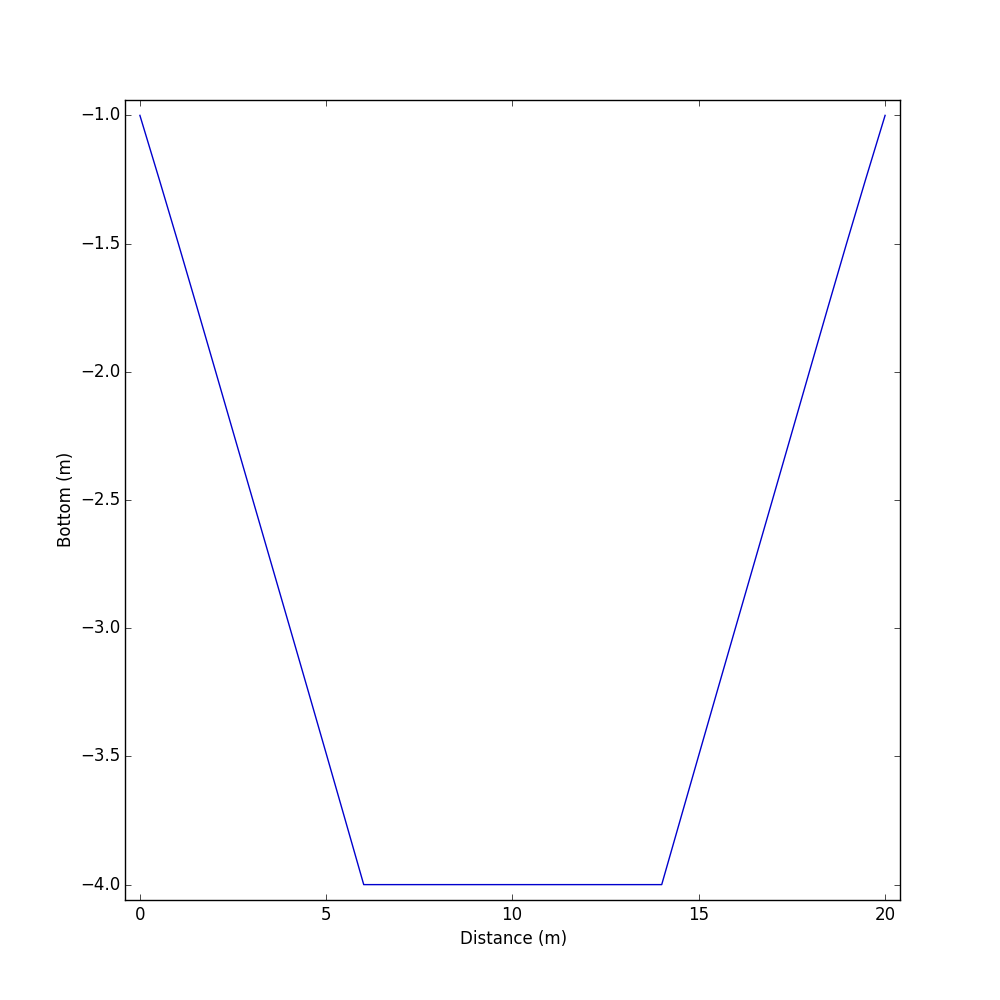
\includegraphics{bathy.png}
 \caption{Wave heigth HM0}
\label{resVeget}
\end{figure}
